\chapter{Implementation}

In this chapter, we first give a high level overview of the possibilities for parallelization and data reuse in the implementation of definition-based cross-correlation algorithm, introduced in section \ref{sec:cross_corr_def}. We then describe an implementation based on Warp Shuffle instructions, with additional optimizations of this implementation. Lastly we implement a solution to the problem of low occupancy for small inputs and go through some additional possibilities for optimization of this implementation.


The definition-based algorithm has several properties which allow for parallelization, optimization through data reuse and distribution of work. Figure \ref{fig:cross_corr_shifts} depicts the output matrix with corresponding relative shift of the two input matrices. As described in Section \ref{sec:cross_corr_opt}, each element of the output matrix can be computed independently in parallel.

\begin{figure}[ht]
	\centering
	\def\svgwidth{\textwidth}
	% Must be relative to current directory
	% as input ignores graphicspath, which is
	% only for includegraphics{}
	\input{./img/overlap-Shifts.pdf_tex}
	\caption{Result matrix with corresponding relative shifts.}
	\label{fig:cross_corr_shifts}
\end{figure}

Each overlap defines a unique set of element pairs which are to be multiplied. Each of these pairs of overlapping elements belongs to exactly one shift of the two matrices.


\section{Parallelization}
In this section, we first highlight the independent parallel tasks present in the definition-based cross-correlation algorithm.  We then define the types of workers which can be derived from CUDA Thread hierarchy, described in Section \ref{sec:thread_hierarchy}. Next we introduce the possible distributions of tasks between different types of workers, with options for data reuse and load balancing.

\subsection{Two matrices}
When we focus on the computation of cross-correlation between two matrices, called \textit{one-to-one} in the rest of the thesis, we can reformulate the definition-based algorithm as a problem with two levels of independent parallel tasks, as can be seen in Figure \ref{fig:cross_corr_one_to_one_tasks}. First level are the different relative shifts of the two input matrices, each represented by a single element in the output matrix. Each of these tasks has a set of independent subtasks corresponding to overlapping pairs of elements of the two input matrices. Each subtask is depicted as a yellow square in Figure \ref{fig:cross_corr_one_to_one_tasks}. Each of these subtasks belongs to exactly one first level task, creating a tree structure. The results of all subtasks of a first level task have to be summed into the result of the parent task. The set of subtasks defines a submatrix in both input matrices, as can be seen in Figure \ref{fig:cross_corr_shifts}.

\begin{figure}[ht]
	\centering
	\def\svgwidth{\textwidth}
	% Must be relative to current directory
	% as input ignores graphicspath, which is
	% only for includegraphics{}
	\input{./img/overlap-Tasks.pdf_tex}
	\caption{Tasks hierarchy in definition-based one-to-one cross-correlation.}
	\label{fig:cross_corr_one_to_one_tasks}
\end{figure}

The goal is to distribute the subtasks between workers in such a way that we maximize parallelism, maximize data reuse and minimize the need for communication and synchronization between workers.

\subsection{Many matrices}

With more than two matrices, we can add additional levels to the task hierarchy shown in \ref{fig:cross_corr_one_to_one_tasks}. As described in Section \ref{sec:cross_corr_forms}, there are several forms of cross-correlation between multiple matrices. For us, the most important of these are:
\begin{enumerate}
	\item \textit{one-to-many},
	\item \textit{n-to-mn},
	\item \textit{n-to-m}.
\end{enumerate}

As we can see, the \textit{one-to-one} type, described in the previous section, together with the \textit{one-to-many} type, are subtypes of the more general \textit{n-to-mn} type. We separate the \textit{one-to-one} and \textit{one-to-many} types as they offer a great possibility for caching the single left matrix.

All of the described types can be partitioned into many \textit{one-to-one} cross-correlations, as can be seen in Figure \ref{fig:cross_corr_many_tasks}. For both \textit{n-to-mn} and \textit{n-to-m} types, the number of green top level tasks, corresponding to the number of result matrices, is equal to $n*m$. To reiterate, the difference \textit{n-to-mn} and \textit{n-to-m} types is that in the \textit{n-to-mn} type, each of the \textit{n} left matrices is cross-correlated with a different set of \textit{m} right matrices, whereas in the \textit{n-to-m} type, all \textit{n} left matrices are cross-correlated with the same \textit{m} right matrices.

\begin{figure}[ht]
	\centering
	\def\svgwidth{0.8\textwidth}
	% Must be relative to current directory
	% as input ignores graphicspath, which is
	% only for includegraphics{}
	\input{./img/overlap-ManyTasks.pdf_tex}
	\caption{Task hierarchy of types with many matrices.}
	\label{fig:cross_corr_many_tasks}
\end{figure}

As in the case of \textit{one-to-one} type, the meaning of the boxes is as follows:

\begin{itemize}
	\item Each green box represents a pair of input matrices, or equivalently a single output matrix;
	\item Each orange box represents an element in the output matrix, or equivalently a relative shift of the two input matrices;
	\item Each yellow box represents a pair of overlapping elements from the two input matrices.
\end{itemize}

All boxes on a given level can be processed completely independently.  Results of the children of a green box have to be written into a single matrix, each into a different element without any collisions. Results of the children of an orange box have to be summed together.

% Segway to data reuse and workers

As the number of tasks cannot be reduced, the only directions for optimization are parallelization and data reuse. Even through tasks can be processed independently and in parallel, many tasks can share and reuse data from other tasks. For example, orange boxes from different subtrees representing the same shift and sharing the same left matrix can be computed by reusing the data from the left matrix. Relations such as this can be used to group tasks for workers to reuse data or pass data to other neighboring workers to reduce the required memory throughput. 

\subsection{CUDA workers}

Section \ref{sec:thread_hierarchy} describes how CUDA threads are hierarchically grouped from smallest to largest as follows:

\begin{enumerate}
	\item thread,
	\item warp,
	\item thread block,
	\item grid.
\end{enumerate}

This thesis provides several implementations of the definition-based cross-correlation algorithm described in following sections, each mapping different level of task hierarchy shown in Figure \ref{fig:cross_corr_many_tasks} to different level of CUDA thread hierarchy.

Based on the choice of the CUDA thread group size, we can utilize smaller groups to compute the subtree of the assigned task, and primitives provided by larger groups to synchronize, communicate and combine results of the tasks between different workers.

\section{Warp shuffle algorithm}
\label{sec:warp_shuffle_alg}

This section describes the implementation of definition-based cross-correlation utilizing Warp Shuffle instructions. We first introduce a simple version of the implementation, later improving it step by step with optimizations evaluated in Section \ref{sec:warp_shuffle_results}.

In the simplified implementation, Warp Shuffle instructions are utilized to shift data loaded from the left matrix and broadcast data loaded from the right matrix between threads in a warp. CUDA threads are used as workers, with each task representing a single relative shift of the two matrices (which is equivalent to a single element of the output matrix), as can be seen in Figure \ref{fig:warp_shuffle_simple_tasks}.

\begin{figure}[ht]
	\centering
	\def\svgwidth{0.5\textwidth}
	% Must be relative to current directory
	% as input ignores graphicspath, which is
	% only for includegraphics{}
	\input{./img/overlap-WarpShuffleSimpleTasks.pdf_tex}
	\caption{Tasks in simple warp shuffle algorithm.}
	\label{fig:warp_shuffle_simple_tasks}
\end{figure}

The main idea behind this algorithm is illustrated in Figure \ref{fig:warp_shuffle_shuffle}. We see how two threads computing shifts $[0,1]$ and $[1,1]$ process elements of the two input matrices. The numbers represent iterations of a \textit{for loop} in the code.

\begin{figure}[ht]
	\centering
	\def\svgwidth{0.7\textwidth}
	% Must be relative to current directory
	% as input ignores graphicspath, which is
	% only for includegraphics{}
	\input{./img/overlap-WarpShuffleShuffle.pdf_tex}
	\caption{Work done by two neighboring threads.}
	\label{fig:warp_shuffle_shuffle}
\end{figure}

As can be seen, the element from the left matrix read by the thread processing shift $[x, y]$ in iteration \textit{i} is required by thread processing shift $[x + 1,y]$ in iteration \textit{i + 1}. This holds for any two neighboring shifts and maps exactly onto the Warp Shuffle Down function, described in Section \ref{sec:thread_cooperation}. When looking at the right matrix in any given iteration, both shifts require the exact same element from the right matrix. This broadcast can be implemented using the general Warp Shuffle function with direct source lane indexing.

% Distribution of shifts between threads and blocks, block dimensions etc.

To utilize these properties, threads of a single warp process 32 consecutive shifts in the \textit{x} axis all with the same \textit{y} axis value, as can be seen in Figure \ref{fig:warp_shuffle_simple_dist}. The \textit{x} axis of \textit{thread block size} is set to \textit{warp size} for simplified grouping of threads into warps. The number of warps per thread block is configurable using a runtime algorithm argument. The grid size is set so that the output matrix is fully covered by threads. Any extra threads are handled by the bound checked reads described next.

% TODO: Maybe show how this solves the problem of first iterations
The problem of iteration \textit{3} in Figure \ref{fig:warp_shuffle_shuffle}, in which the lower thread does not have any value to compute, can be solved in several ways. If we were programming for a CPU, we would give the two for loops implementing the two worker threads different bounds so that the second worker stops earlier. A more GPU friendly implementation needs to prevent thread divergence. This is achieved by executing the range check only once when loading the data from the left matrix into a register of the thread. If the thread is loading value outside the matrix, it loads 0 instead. This makes the result of the multiplication performed in each step 0 which is then added to the sum, making it effectively a \textit{noop} instruction while preventing thread divergence. This also handles any extra threads introduced due to the fixed size of thread block and overlap sizes not divisible by warp size.

\begin{figure}[ht]
	\centering
	\def\svgwidth{0.8\textwidth}
	% Must be relative to current directory
	% as input ignores graphicspath, which is
	% only for includegraphics{}
	\input{./img/overlap-WarpShuffleWarps.pdf_tex}
	\caption{Distribution of shifts between CUDA threads, warps and blocks.}
	\label{fig:warp_shuffle_simple_dist}
\end{figure}

\subsection{Algorithm steps}

The following description assumes \textit{warp size} to be 32, as is the case for all existing Nvidia GPUs. To utilize coalesced loading from global memory, the left buffer shuffled between threads is split into two parts of 32 items each, which together function as a single 64 item ring buffer. As described above, any out of bounds loads are range checked and load value 0 instead using code such as this::
\begin{lstlisting}[
style=cuda
]

template<typename T>
__device__ T load_with_bounds_check(const T* source, int idx, size_t size) {
	return (idx >= 0 && idx < size) ? source[idx] : 0;
}
\end{lstlisting}


When loading the buffer, bound checked load shown above is used to load 32 consecutive values (or 0 if out of bounds), storing one item per thread into a register. This is implemented by the following code:
\begin{lstlisting}[
style=cuda
]

T thread_left_bottom = load_with_bounds_check(
	left_row,
	warp_x_left + warp.thread_rank(),
	matrix_size.x
);

\end{lstlisting}

As we can see, each thread holds single value of \texttt{thread\_left\_bottom}. Same is done for \texttt{thread\_left\_top}, creating a 64 item ring buffer distributed between threads of a warp which is shifted using the Warp Shuffle instructions.

The algorithm can be described by the following pseudocode:

\begin{lstlisting}[]
COMPUTE warp overlap bounds
COMPUTE thread output position

SET sum = 0
FOR each overlapping row
	bound checked load of thread_left_bottom

	FOR every 32nd item in overlap row
		bound checked load of thread_left_top
		bound checked load of thread_right

		run 32 iterations of main loop
	ENDFOR
ENDFOR

IF thread output not out of bounds
	write sum to output
\end{lstlisting}

We compute bounds for the union of overlaps processed by the threads of the warp. The union of overlaps gives us a submatrix of the right matrix, which we then iterate over using the two nested for loops. When loading from the left matrix, each thread uses its assigned shift derived from the output position to read the correct element of the left matrix. As threads of a warp compute shifts which have the same \textit{y} axis and are sequential in the \textit{x} axis, the bound-checked loads of the left buffer result in sequential coalesced reads. As the loads of the right buffer are bound checked from the bottom by the overlap bounds, the bound-checked reads are utilized only in the last iteration when the size of the overlap is not divisible by warp size. We go through each row of the overlap in steps of 32 as that is the number of items processed by the main loop, based on the number of threads in a warp.


The main body of the algorithm is a for loop with 32 iterations, where in iteration $i$ we broadcast right value from thread $i$ and each thread multiplies this value with the value from the bottom left buffer stored by this thread. We then shift the left buffer using two warp shuffle instructions. After 32 steps, the top part of the left buffer is now in the bottom part of the left buffer and all the values from right buffer have been broadcast, allowing us to go ahead with the next iteration of the loop over row items.

The main loop is illustrated by the following code:

\begin{lstlisting}[
style=cuda
]

for (size_t i = 0; i < warp.size(); ++i) {
	// Broadcast right buffer
	auto right_val = warp.shfl(thread_right, i);
	sum += thread_left_bottom * right_val;

	// Shift left buffer

	// General shuffle does module on source lane argument
	// Thread 0 needs to connect the top buffer to the bottom buffer
	thread_left_bottom = warp.shfl(
		warp.thread_rank() != 0 ? thread_left_bottom : thread_left_top,
		warp.thread_rank() + 1
	);
	thread_left_top = warp.shfl_down(thread_left_top, 1);
}
\end{lstlisting}


\subsection{Work distribution}
\label{sec:warp_shuffle_work_dist}

In the simplified algorithm described above, there are massive differences in work done by different threads. As we can see in Figure \ref{fig:warp_shuffle_work_difference}, the thread processing the left overlap has much less work than the thread processing the right overlap. This will lead to problems with occupancy once the threads with small amount of work are completed.

\begin{figure}[ht]
	\centering
	\def\svgwidth{0.6\textwidth}
	% Must be relative to current directory
	% as input ignores graphicspath, which is
	% only for includegraphics{}
	\input{./img/overlap-WarpShuffleWorkDifference.pdf_tex}
	\caption{Task size difference in the simplified algorithm.}
	\label{fig:warp_shuffle_work_difference}
\end{figure}

To distribute the work more evenly, we need to change what is considered a task processed by a worker. Compared to the simplified implementation, where task represents the whole overlap defined by the given shift, with work distribution a task represents several full continuous rows of overlapping pairs of elements (yellow boxes), as can be seen in figure \ref{fig:warp_shuffle_work_dist_tasks}. With this change, multiple workers may write to the same element in the output matrix. Each worker must add the final sum of the assigned task to sums of all other workers processing tasks of the same shift. As each worker needs to add the sum just once, utilizing the \textit{atomicAdd} operation on the output matrix in global memory is sufficient. It also allows us greater freedom of assigning tasks to workers across the whole grid compared to grouping workers for the given shift into a thread block, which would be required to utilize shared memory for communication. The maximum number of rows in a task is provided as a run-time argument to the algorithm, and influences the number of workers created.

\begin{figure}[ht]
	\centering
	\def\svgwidth{0.8\textwidth}
	% Must be relative to current directory
	% as input ignores graphicspath, which is
	% only for includegraphics{}
	\input{./img/overlap-WarpShuffleWorkDistTasks.pdf_tex}
	\caption{Tasks in warp shuffle algorithm with load balancing.}
	\label{fig:warp_shuffle_work_dist_tasks}
\end{figure}


We provide several algorithms to derive the number of workers started and the mapping from thread ID to the row of the output matrix and the worker rank for given row. The provided algorithms are:

\begin{itemize}
	\item None,
	\item Rectangle,
	\item Triangle.
\end{itemize}


The algorithms are illustrated in Figures \ref{fig:work_dist_max_1} and \ref{fig:work_dist_max_2}. In these, the purple boxes represent number of tasks for each shift in the given row of the output matrix. Each task represents given number of full continuous rows of the overlap. For Figure \ref{fig:work_dist_max_1}, each purple box represents a single row of the overlap, or in other words, purple boxes represent number of overlapping rows for each shift in given output matrix row. As we define work distribution based on number of overlapping rows, worker ID is the \textit{y} axis of the thread ID, i.e. $blockIdx.y * gridSize.y + threadIdx.y$. This means that all threads with the given value of \textit{y} axis share the same worker ID. Due to the way we utilize Warp Shuffle instruction to shift values along the \textit{x} axis, i.e. along each row, the distribution of work into tasks takes into account only the number of rows, not the size of each row, as can be seen in Figure \ref{fig:warp_shuffle_work_dist_tasks}. 


\subsubsection{None distribution}		
The \textit{None} distribution is provided mainly to measure the overhead of the code changes required to implement work distribution. This distribution behaves identically to the simplified algorithm with no distribution. As such, it starts a single worker for each shift in the output matrix. The workers are assigned by directly mapping their \textit{y} axis ID to the row of the output matrix.

\subsubsection{Rectangle distribution}

The \textit{Rectangle} distribution computes $m$, the maximum number of tasks required for any shift, and starts $m$ workers for all shifts, creating a rectangle of workers which can be seen in Figure \ref{fig:work_dist_max_1}. The redundant workers are stopped immediately after work assignment. To start the required number of workers, the \textit{y} axis of grid size is multiplied by $m$.
The tasks are assigned using $worker\_ID \mod output\_matrix\_size.y$ with worker rank computed as $worker\_ID / output\_matrix\_size.y$.

\subsubsection{Triangle distribution}
The \textit{Triangle} distribution starts exactly one worker for each task. The disadvantage of this distribution is the complex computation required to assign workers to tasks. This computation includes many multiplications, divisions and most importantly a low throughput square root instruction. For inputs where the size of each task is small, the overhead of triangle distribution may be greater than any gains provided by load balancing and increased occupancy due to work distribution. The grid size is increased to start at least the required number of workers, with some overallocation due to the fixed size of thread blocks. To map worker ID to output matrix row and worker rank, we use the following formula, which computes the worker ID $i$ of the worker at the start of the triangle row $x$:

\[
	r*x^2 - (3r - t)*x + (2r - t) = i
\]

where $r$ is the algorithm argument \textit{maximum number of rows per worker}, $t$ is the number of workers on the top row of the triangle, $x$ is workers row in the triangle, corresponding to worker rank, and $i$ is worker ID. Solved for $x$, we get the following formula:

\[
	x = floor(\frac{(3r - t) + \sqrt{(3r - t)^2 - 4r(2r - t - i)}}{2r})
\]

which is the positive solution of the quadratic equation rounded down. For any worker ID on the row $x$, this formula will return $x$ when given worker ID $i$.

Lastly, we need to compute the variable $t$, the number of items on the top row of the triangle. The number of items on the top row can be computed as:
\[
	output\_matrix\_size.y \mod (2*r)
\].


\begin{figure}[ht]
	\centering
	\def\svgwidth{\textwidth}
	% Must be relative to current directory
	% as input ignores graphicspath, which is
	% only for includegraphics{}
	\input{./img/overlap-DistMax1Row.pdf_tex}
	\caption{Work distribution of 4x4 input with 1 row per task.}
	\label{fig:work_dist_max_1}
\end{figure}


\begin{figure}[ht]
	\centering
	\def\svgwidth{\textwidth}
	% Must be relative to current directory
	% as input ignores graphicspath, which is
	% only for includegraphics{}
	\input{./img/overlap-DistMax2Rows.pdf_tex}
	\caption{Work distribution of 4x4 input with maximum of 2 rows per task.}
	\label{fig:work_dist_max_2}
\end{figure}


\subsection{Utilizing multiple right matrices}
\label{sec:multimat_right}

Another problem of the simplified implementation not solved by work distribution, described in Section \ref{sec:warp_shuffle_work_dist}, is the ratio of warp shuffle instructions to arithmetic instructions. For each multiplication and addition, represented by a single yellow box, we must execute three warp shuffle instructions. This makes warp shuffle instructions the bottleneck in the simplified implementation, as can be seen in Figure \ref{fig:executed_instructions_multiright}. The warp shuffle instructions (SHFL) dominate the executed instruction mix, which results in 97\% utilization of the \textit{LSU} pipeline implementing the shuffle instructions, as can be seen in Figures \ref{fig:pipeline_utilization_multiright}. Compare this to the fused multiply-add instructions (FFMA) implementing the multiplication and addition, which is implemented by the \textit{FMA} pipeline with less than 10\% utilization for the simplified algorithm.


There are several ways to improve the ratio of warp shuffle instructions to the fused multiply-add instructions. The simplest way is to utilize the \textit{one-to-many} type of computation, and let each worker compute cross-correlation between one left matrix and many right matrices at once. We call this the \textit{multimat\_right} optimization. The obvious advantage is data reuse, as the data from the left matrix is used to compute multiple results. The main advantage is that each additional right matrix only adds a single warp shuffle instruction, while also adding one fused multiply-add instruction. The ratio of warp shuffle to fused multiply-add instructions can then be expressed as $2 + r : r$, where $r$ is the number of shifts (from $r$ right matrices) computed by each worker, which for any value greater than $1$ is much improved from the $3:1$ ratio of the simplified warp shuffle algorithm.

The effects of this optimization can be seen in Figures \ref{fig:executed_instructions_multiright} and \ref{fig:pipeline_utilization_multiright}. These figures compare the simplified algorithm against the optimized algorithm using 8 right matrices per worker on input of size 256x256 with 1 left matrix and 16 right matrices. As we can see, the \texttt{LSU} pipeline is still a bottleneck even for the optimized algorithm, but the utilization of the \texttt{FMA} pipeline, which does the useful part of the computation, has increased from 9\% to 20\%. The most visible change is in the mix of the executed instructions, where we see a very noticeable improvement in the ratio of shuffle instructions (SHFL) to the floating point fused multiply-add instructions (FFMA). As expected, the ratio improves from $3 : 1$ to $10 : 8$. The small improvement in the \texttt{LSU} pipeline utilization can be explained by the comparatively low throughput of the warp shuffle instructions compared to the fused multiply-add instructions. This is exacerbated by our use of Compute Capability 7.5 card for profiling, which has half the warp shuffle throughput of all other Compute Capabilities.

% TODO: Benchmark on gpulab

\begin{figure}[ht]
	\centering
	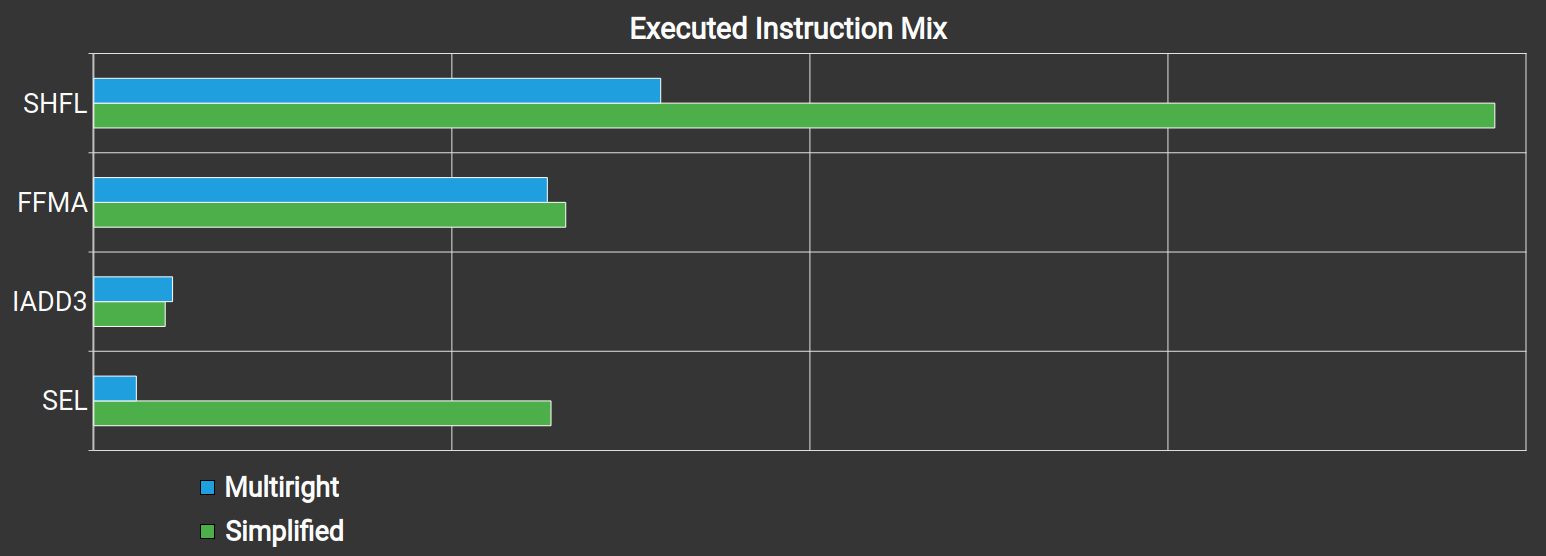
\includegraphics[width=\textwidth]{executed_instructions_multiright.png}
	\caption{Comparison of instruction mix between \textit{one-to-many} simplified algorithm and the multiple right matrix optimization.}
	\label{fig:executed_instructions_multiright}
\end{figure}

\begin{figure}[ht]
	\centering
	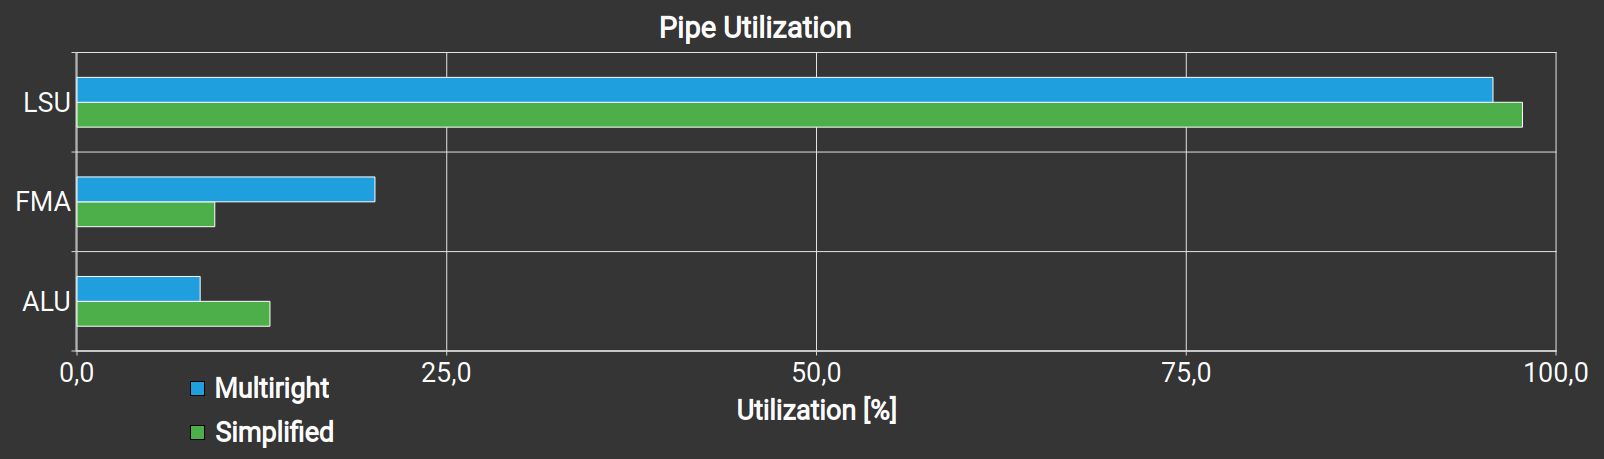
\includegraphics[width=\textwidth]{pipeline_utilization_multiright.png}
	\caption{Comparison of pipeline utilization between \textit{one-to-many} simplified algorithm and the multiple right matrix optimization.}
	\label{fig:pipeline_utilization_multiright}
\end{figure}



% TODO: Benchmark results

\subsection{Multiple rows from the right matrix}
\label{sec:multirow_right}

Another way to improve the instruction ratio is to process multiple rows from the same right matrix, which can be used even for the \textit{one-to-one} type of computation. We call this the \textit{multirow\_right} optimization. There are several caveats when implementing this optimization. The main difference is that a single thread now computes multiple different shifts instead of the same shift in multiple matrices, as is done by the \textit{multimat\_right}. These shifts differ in the \textit{y} axis, and represent consecutive elements in a column of the output matrix, as can be seen in Figure \ref{fig:multirow_shifts}. Each of these shifts represents different overlap of the two input matrices, requiring different bounds in the \textit{y} axis.

\begin{figure}[ht]
	\centering
	\def\svgwidth{\textwidth}
	% Must be relative to current directory
	% as input ignores graphicspath, which is
	% only for includegraphics{}
	\input{./img/overlap-Multirow.pdf_tex}
	\caption{Shifts assigned to workers by the \textit{multirow\_right} algorithm with 4 shifts per worker.}
	\label{fig:multirow_shifts}
\end{figure}

Due to these different bounds for the shifts computed by the worker, we have to add explicit initialization and finalization code which handles the case where the current row being processed from the left matrix overlaps with the right matrix in a subset of shifts computed by the worker, as can be seen in Figure \ref{fig:multirow_init}. This figure shows a run of the algorithm with three shifts per worker. For threads which compute shifts with top of the right matrix (in red) inside the left matrix (in blue), i.e. shift with a positive \textit{y} axis, or where the top of the right matrix is less than $number\_of\_shifts\_per\_thread$ above left matrix, i.e. $y < 0$ and $y > -number\_of\_shifts\_per\_thread$, we must run separate initialization steps. These can be seen in Figure \ref{fig:multirow_init}, where the first row processed from the left matrix overlaps in only a single shift computed by the thread, second row overlaps in two shifts and rest overlap in all three shifts. As such, we first run initialization step which processes a single row, after which we run an initialization step processing two rows. The maximum number of initialization steps is equal to $number\_of\_shifts\_per\_thread - 1$. If the top of the right matrix is outside the left matrix, i.e. the shifts computed by the thread have negative \textit{y} axis, with $y0 = min(y)$ being the minimum vertical shift, the first $abs(y0)$ initialization steps are skipped. 

Similar problem is present when thread computes shifts in which the bottom of the right matrix is inside the left matrix, i.e. $y < 0$, or less than $number\_of\_shifts\_per\_thread$ below the left matrix, i.e. $y > 0$ and $y < number\_of\_shifts\_per\_thread$. This situation is illustrated in Figure \ref{fig:multirow_fini}.

\begin{figure}[ht]
	\centering
	\def\svgwidth{0.5\textwidth}
	% Must be relative to current directory
	% as input ignores graphicspath, which is
	% only for includegraphics{}
	\input{./img/overlap-MultirowInit.pdf_tex}
	\caption{Initial steps of the \textit{multirow\_right} algorithm.}
	\label{fig:multirow_init}
\end{figure}

\begin{figure}[ht]
	\centering
	\def\svgwidth{0.5\textwidth}
	% Must be relative to current directory
	% as input ignores graphicspath, which is
	% only for includegraphics{}
	\input{./img/overlap-MultirowFinalize.pdf_tex}
	\caption{Final steps of the \textit{multirow\_right} algorithm.}
	\label{fig:multirow_fini}
\end{figure}

After the initialization phase is finished, the main loop is conceptually very similar with the multiple right matrices case described previously. The only major differences are the accumulation of the final result through shared memory instead of registers and the reversal of the results for given row group.

The complexity of the code forces us to share the results of different function calls, such as the initialization, main body and finalization, through shared memory. We allocate a shared memory array with size $max\_shifts\_per\_thread * thread\_block\_size$, which is used to accumulate the final result of all shifts for all threads of the thread block. This array can be seen in Figure \ref{fig:multirow_sharedmem}. The array begins with the first shift of each thread of the thread block, then second shift of each thread of the thread block, up to shift $max\_shifts\_per\_thread$, which is an algorithm argument. As all threads of a warp compute the same number of shifts, this ordering ensures access to shared memory causes no bank conflicts.

\begin{figure}[ht]
	\centering
	\def\svgwidth{0.5\textwidth}
	% Must be relative to current directory
	% as input ignores graphicspath, which is
	% only for includegraphics{}
	\input{./img/overlap-MultirowSharedmem.pdf_tex}
	\caption{Shared memory allocation to threads.}
	\label{fig:multirow_sharedmem}
\end{figure}

When storing the result of main loop iteration into the shared memory array, we must reverse the results as can be seen in Figure \ref{fig:multirow_reversal}. Multiple rows loaded from the right matrix are ordered as they are loaded from the matrix, indexing them $0$ to $n$. As we can see, the shift in which given row from right matrix overlaps the row from the left matrix is given by $n - i$, which requires us to inverse the index when storing the result into shared memory. This needs to also be done during initialization and finalization steps, which is another reason why results need to be accumulated through shared memory, as we need to pass only the last $s$ shifts to the step \texttt{Finish s}, for which the simplest implementation is pointer arithmetic on the shared memory array.

\begin{figure}[ht]
	\centering
	\def\svgwidth{0.7\textwidth}
	% Must be relative to current directory
	% as input ignores graphicspath, which is
	% only for includegraphics{}
	\input{./img/overlap-MultirowInversion.pdf_tex}
	\caption{Reversal of results when accumulating to shared memory.}
	\label{fig:multirow_reversal}
\end{figure}

One of the disadvantages of this algorithm is the repeated reading of the same rows of the right matrix by each worker. As we already go through each row by shuffling from left to right, there is no simple way to reuse rows from top to bottom as we compute the overlap for given shifts. With 3 shifts per worker, each row of the right matrix processed by the main loop is read 3 times, once for each of the shifts processed by the worker. Each time, it is used with different left row. In the \textit{multimat\_right} optimization, these repeated reads are done by different workers, making them parallel and improving occupancy. This can be improved by additionally utilizing multiple left rows during the computation, reducing the number of times the rows from the right matrix need to be reread. This implementation is described in Section \ref{sec:multirow_both}.


When profiling this optimization, as shown in Figures \ref{fig:executed_instructions_multirow} and \ref{fig:pipeline_utilization_multirow}, we can see similar improvements as with the previous \textit{multiright} optimization. We have to keep in mind that the \textit{multirow\_right} algorithm improves the \textit{one-to-one} type of computation, which cannot be improved by the previous optimization. We can also combine these two optimizations, described in Section \ref{sec:combining_optimizations}. As before, the \textit{LSU} pipeline remains a bottleneck, but the utilization of \textit{FMA} pipeline is improved from 9\% to 17\%. With 4 shifts per worker, the ratio improves from $3 : 1$ to $6 : 4$ as expected from the $2 + r : r$ theoretical ratio. As this optimization improves the \textit{one-to-one} computation, it is more sensitive to occupancy reduction when workers process more than one shift, mainly due to the smaller input size compared to the \textit{one-to-many} computation.

\begin{figure}[ht]
	\centering
	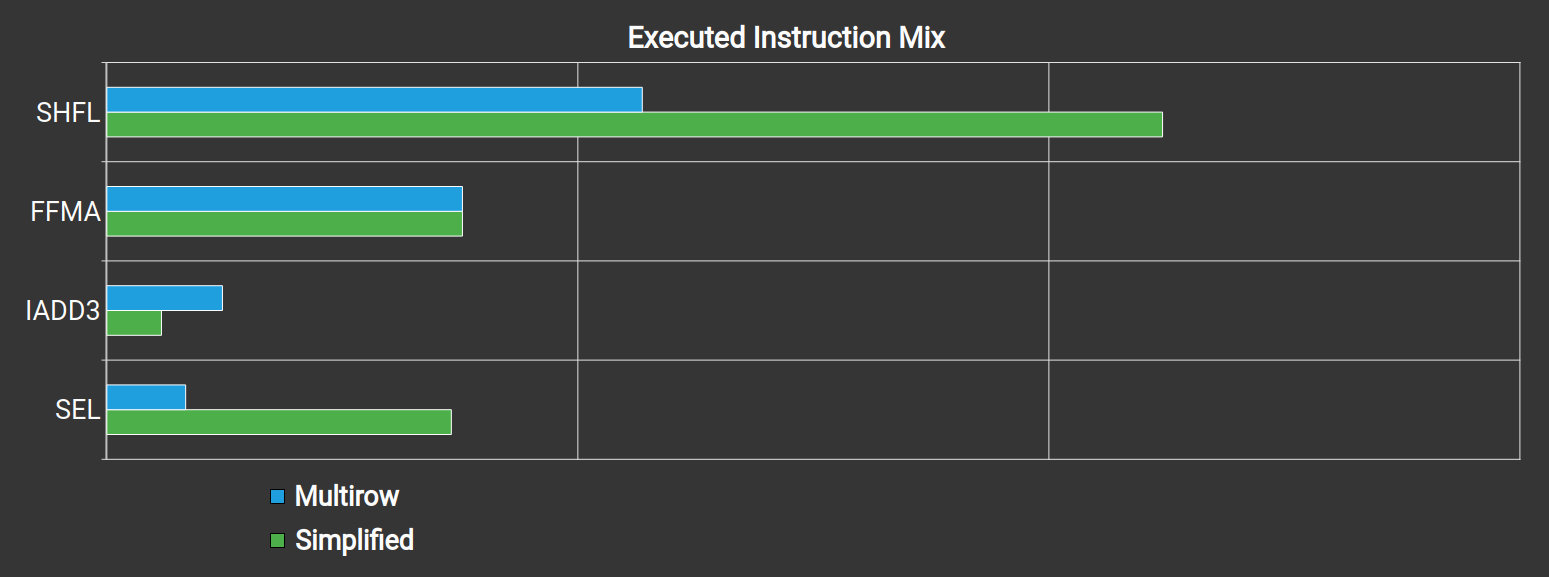
\includegraphics[width=\textwidth]{executed_instructions_multirow.png}
	\caption{Comparison of instruction mix between \textit{one-to-one} simplified algorithm and the \textit{multirow\_right} optimization.}
	\label{fig:executed_instructions_multirow}
\end{figure}

\begin{figure}[ht]
	\centering
	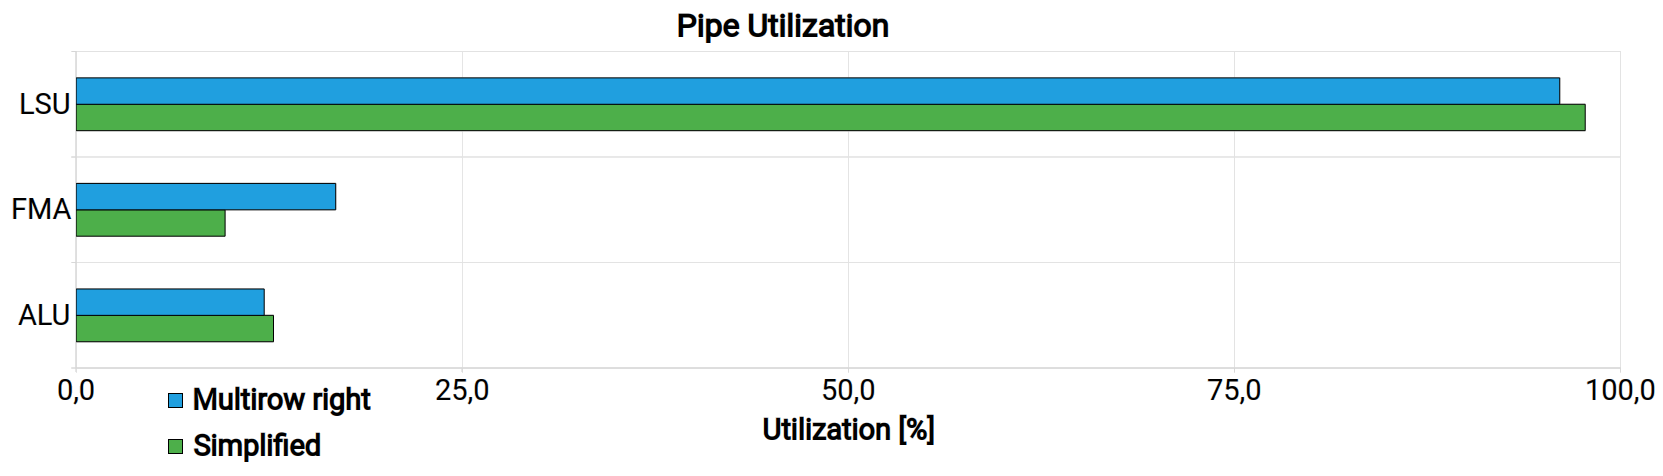
\includegraphics[width=\textwidth]{pipeline_utilization_multirow.png}
	\caption{Comparison of pipeline utilization between \textit{one-to-one} simplified algorithm and the \textit{multirow\_right} optimization.}
	\label{fig:pipeline_utilization_multirow}
\end{figure}


% TODO: Computing with double

% https://forums.developer.nvidia.com/t/loop-through-register-array-without-using-local-memory/29458/3
\section{Advanced warp shuffle optimizations}

The optimizations of the warp shuffle algorithm described up to this point hint at further possibilities, such as using multiple left matrices and multiple rows from the left matrix in combination with the already described optimizations. This section first introduces the Local array optimization done by the \textit{nvcc} compiler, on which our implementations heavily rely. Next we describe the problem with the \textit{nvcc} compiler not performing the Local array optimization with our solution to this problem. We then utilize this solution to implement two further optimizations, which extend and are combined with the basic optimizations described in Section \ref{sec:warp_shuffle_alg}. Lastly we illustrate the effects of the Local array optimization on the implemented solutions.


\subsection{Local array optimization}
\label{sec:local_array_optimization}

% Why is it important that the arrays are in registers
% https://developer.nvidia.com/blog/fast-dynamic-indexing-private-arrays-cuda/
The \textit{multimat\_right} and \textit{multirow\_right} optimizations heavily rely on the CUDA compiler to place arrays such as the following into registers:

\begin{lstlisting}[
style=cuda
]
template<size_t NUM_RIGHTS, typename T, typename RES>
__device__ void warp_shuffle_impl(...) {
...
	RES sum[NUM_RIGHTS];
	for (size_t r = 0; r < NUM_RIGHTS; ++r) {
		sum[r] = 0;
	}
...
	T thread_right[NUM_RIGHTS];
	for (size_t r = 0; r < NUM_RIGHTS; ++r) {
		thread_right[r] = load_with_bounds_check(...);
	}
...
}
\end{lstlisting}

If an array is small and only accessed using static indexing, where all indices are known constants at compile time, the CUDA compiler places all elements of the array into registers.  % TODO: Quote the blog
This allows for very fast access without placing any additional strain on the \textit{LSU} pipeline. The array can also be accessed in small for loops with known compile time bounds, which are unrolled by the compiler and again result in static indexing. If for any access the index cannot be computed during compile time, the whole array is placed into Local memory, described in Section \ref{sec:memory_hierarchy}. Local memory is part of the device memory, and as such is the slowest memory accessible from device code. Each access also utilizes the \textit{LSU} pipeline, interfering with the warp shuffle instructions. 



\subsection{Advanced optimizations and local arrays}
\label{sec:local_array_optimization_code_changes}

When implementing the \textit{multimat\_both} and \textit{multirow\_both} optimizations, described in Sections \ref{sec:multimat_both} and \ref{sec:multirow_both} respectively, we encountered a problem with the \textit{nvcc} compiler not optimizing the local arrays into registers. 

Using profiling and by examining the SASS, we isolated the problem to the \textit{thread\_left\_bottom} and \textit{thread\_left\_top} arrays. We further isolated it to the following part of the code, which in its original form shared by the simplified, \textit{multimat\_right} and \textit{multirow\_right} implementations looks like this:

\begin{lstlisting}[
style=cuda
]
thread_left_bottom = warp.shfl(
	warp.thread_rank() != 0 ? thread_left_bottom : thread_left_top,
	warp.thread_rank() + 1
);
thread_left_top = warp.shfl_down(thread_left_top, 1);
\end{lstlisting}

To process multiple values from a single or multiple left matrices, the code needs to be changed into the following:

\begin{lstlisting}[
style=cuda
]
#pragma unroll
for (dsize_t l = 0; l < NUM_LEFTS; ++l) {
	thread_left_bottom[l] = warp.shfl(
		warp.thread_rank() != 0 ? thread_left_bottom[l] : thread_left_top[l],
		warp.thread_rank() + 1
	);
	thread_left_top[l] = warp.shfl_down(thread_left_top[l], 1);
}
\end{lstlisting}

The \textit{nvcc} compiler should be able to unroll this loop, and thanks to static indexing, the \textit{thread\_left\_bottom} and \textit{thread\_left\_top} local arrays should be optimized into registers. Unfortunately, as we can see in Figure \ref{fig:local_memory_load_sass}, the compiler behaves as if dynamic indexing was used and pulls the arrays into local memory. 
Due to the closed source nature of the \textit{nvcc} compiler, we can only speculate on the reasons why this version worked while the other versions did not. One possibility, based on the generated SASS instructions seen in Figure \ref{fig:local_memory_load_sass}, is that the ternary operator is optimized into dynamic array indexing, which then prevents the local array optimization. As there is no visible branching in the unrolled loop, the base address of either the \textit{thread\_left\_bottom} or the \textit{thread\_left\_top} is loaded into register R65, which is then reused in all loads, resulting in dynamic indexing. 

\begin{figure}[ht]
	\centering
	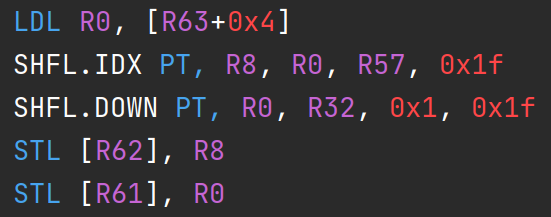
\includegraphics[width=0.7\textwidth]{local_memory_load_sass.png}
	\caption{The loop body SASS instructions with local memory access.}
	\label{fig:local_memory_load_sass}
\end{figure}

We experimented with several solutions, with the following version compiling into static indexing:

\begin{lstlisting}[
style=cuda
]
#pragma unroll
for (dsize_t l = 0; l < NUM_LEFTS; ++l) {
	T bottom_shift_val;
	if (warp.thread_rank() != 0) {
		bottom_shift_val = thread_left_bottom[l];
	} else {
		bottom_shift_val = thread_left_top[l];
	}

	thread_left_bottom[l] = warp.shfl(bottom_shift_val, warp.thread_rank() + 1);
	thread_left_top[l] = warp.shfl_down(thread_left_top[l], 1);
}
\end{lstlisting}


\begin{figure}[ht]
	\centering
	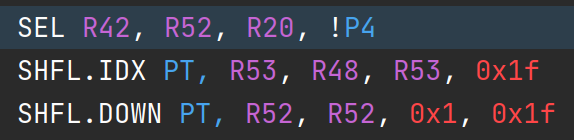
\includegraphics[width=0.7\textwidth]{sass_no_local_mem.png}
	\caption{The updated loop body SASS instructions with no local memory access.}
	\label{fig:sass_no_local_memory}
\end{figure}

As we can see in Figure \ref{fig:sass_no_local_memory}, the body of the updated loop results in a single \textit{SEL} instruction which selects the top or the bottom part of the buffer. This version of the loop is used by the advanced warp shuffle optimizations described in the following sections.

\subsection{Multiple left matrices}
\label{sec:multimat_both}

A natural step following the use of multiple right matrices is to also utilize multiple left matrices. This can only be used in the \textit{n-to-m} computation type, as the \textit{n-to-mn} type and its subtypes correlate each left matrix with a different set of right matrices.

The changes to the code of the \textit{multimat\_right} optimization are straight forward. We add additional template parameter \textit{NUM\_LEFTS} to the implementing function and change both \textit{thread\_left\_bottom} and \textit{thread\_left\_top} from simple variables into local arrays, as was done for the \textit{thread\_right} variable by the \textit{multimat\_right} optimization. The number of shifts computed by each thread is also changed to $NUM_LEFTS * NUM_RIGHTS$ from only $NUM_RIGHTS$. 


This optimization improves the ratio of warp shuffle to fused multiply-add instructions to $ 2 * l + r : l * r$, where $l$ is the number of left matrices and $r$ the number of right matrices utilized by each worker. This improvement can be seen in the executed instruction mix shown in Figure \ref{fig:shuffle_multimat_both_instruction_mix}. 

\subsection{Multiple rows from both matrices}
\label{sec:multirow_both}

When improving \textit{one-to-one} computation using the \textit{multirow\_right} optimization described in Section \ref{sec:multirow_right}, which processes multiple rows from the same right matrix, we described a further improvement using multiple rows from the left matrix. This not only further improves the ratio of warp shuffle to fused multiply-add instructions, but also reduces the number of times every row from the right matrix is reread. 

The initialization and finalization parts are left unchanged. The main difference is that the main loop now advances not by a single left row, but by the number of left rows given by the algorithm argument. We also need to add an additional stage between the main loop and finalization, where we utilize the original single step main loop to finish the leftover rows from the left matrix. This step is required when the number of left rows in the overlap is not divisible by the number of left rows processed in each iteration of the new multi-step main loop.

The algorithm parameters are changed from just the number of right rows to be processed by each thread to a pair of parameters, the number of left rows to process in each iteration of the main loop and the number of shifts to be processed by each thread. In the \textit{multirow\_right} algorithm, the number of shifts per thread was equal to the number of right rows to be processed by each thread. For clarity, we now invert this relationship, explicitly providing number of shifts and deriving the number of right rows to be loaded from the number of shifts and the number of left rows. 

In each iteration of the main loop, the left row 0 is processed with right rows $[0, NUM\_SHIFTS - 1]$, left row 1 with right rows $[1, NUM\_SHIFTS]$ and left row \textit{l} with right rows $[l, NUM\_SHIFTS - 1 + l]$. As such, we load $NUM\_SHIFTS + NUM_LEFT_ROWS - 1$ right rows, so that we can process all the left rows simultaneously. 

The ratio of warp shuffles to fused multiply-adds for this optimization is $l + (s - 1 + l) : l * s$ in the main loop, where $l$ is the number of left rows processed by each iteration of the main loop and $s$ is the number of shifts processed by each thread.  
The initialization, single step main loop and finalization share the original ratio of the \textit{multirow\_right} implementation. This ratio can be seen in Figure \ref{fig:shuffle_multirow_both_instruction_mix}.


\subsection{Effects of local array optimization}

In this section, we compare the \textit{multimat\_both} and \textit{multirow\_both} algorithms with and without the local array optimization, described in Section \ref{sec:local_array_optimization}. The only difference between the versions is described in Section \ref{sec:local_array_optimization_code_changes}, with a change to the loop shuffling the buffers containing data from the left matrices.

We can clearly see the additional local memory store (STL) and load (LDL) instructions in the instruction mix in Figures \ref{fig:shuffle_multimat_both_instruction_mix} and \ref{fig:shuffle_multirow_both_instruction_mix}. Apart from these, we can see that the number of remaining instructions is the same.

\begin{figure}[ht]
	\centering
	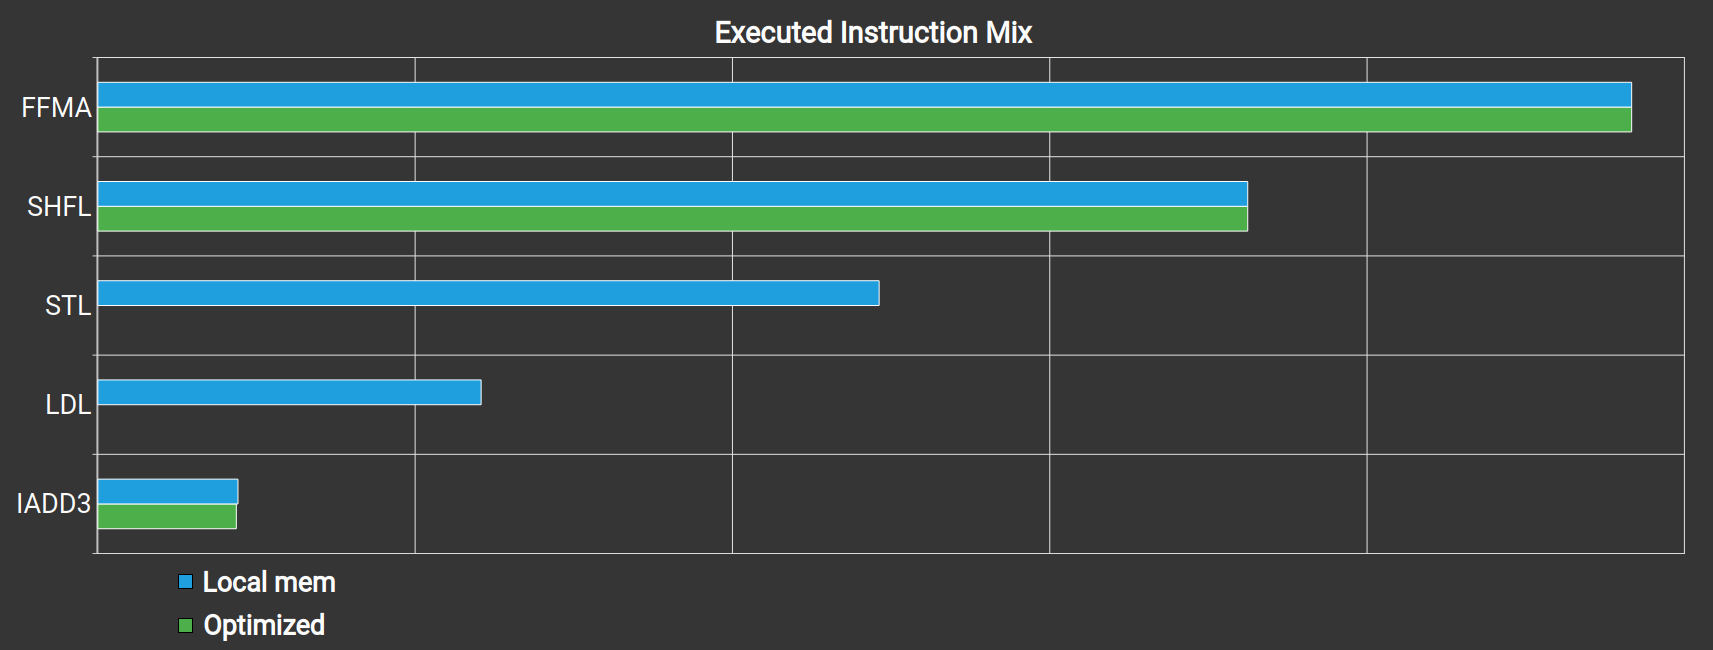
\includegraphics[width=0.7\textwidth]{executed_instructions_shuffle_multimat_both.png}
	\caption{Instruction mix of the \textit{multimat\_both} optimization with local memory.}
	\label{fig:shuffle_multimat_both_instruction_mix}
\end{figure}


\begin{figure}[ht]
	\centering
	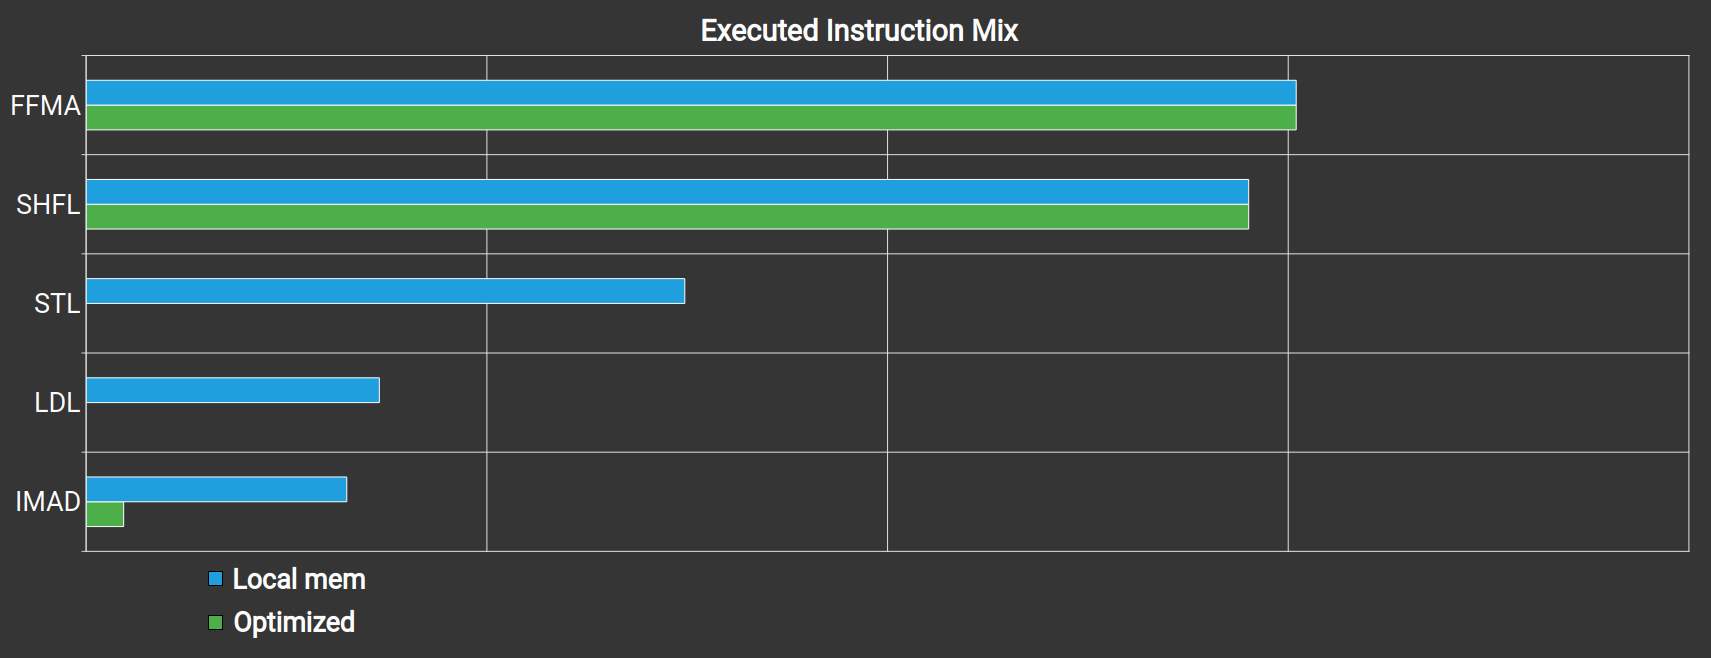
\includegraphics[width=0.7\textwidth]{executed_instructions_shuffle_multirow_both.png}
	\caption{Instruction mix of the \textit{multirow\_both} optimization with local memory.}
	\label{fig:shuffle_multirow_both_instruction_mix}
\end{figure}



When comparing the runtime of each implementation, the difference is even more noticeable. As we can see in both Figure \ref{fig:multimat_both_speedup} and Figure \ref{fig:multirow_both_speedup}, the speedup for smaller sizes is limited due to low occupancy, but is still present. Figure \ref{fig:multimat_both_speedup} shows that for matrices of size 64 by 64, the solution without local memory access is already 2 times faster. 
Figure \ref{fig:multirow_both_speedup} shows that there is slightly smaller improvement in the \textit{multirow\_both} optimization compared to the \textit{multimat\_both}. This is most likely caused by the initialization and finalization parts of the implementation, together with greater overall complexity of the optimization.
% TODO: Rearange the graphs to be next to each other in a single figure
\begin{figure}[ht]
	\centering
	\def\svgwidth{0.5\textwidth}
	% Must be relative to current directory
	% as input ignores graphicspath, which is
	% only for includegraphics{}
	\input{./img/multimat_speedup.pdf_tex}
	\caption{Improvement of the \textit{multimat\_both} optimization without Local memory access.}
	\label{fig:multimat_both_speedup}
\end{figure}

\begin{figure}[ht]
	\centering
	\def\svgwidth{0.5\textwidth}
	% Must be relative to current directory
	% as input ignores graphicspath, which is
	% only for includegraphics{}
	\input{./img/multirow_speedup.pdf_tex}
	\caption{Improvement of the \textit{multirow\_both} optimization without Local memory access.}
	\label{fig:multirow_both_speedup}
\end{figure}


\subsection{Combining the optimizations}
\label{sec:combining_optimizations}

We have implemented the following optimizations of the Warp Shuffle algorithm:

\begin{itemize}
	\item work distribution,
	\item multiple right matrices per worker (\textit{multimat\_right}),
	\item multiple rows from each right matrix per worker (\textit{multirow\_right}),
	\item multiple left matrices per worker (\textit{multimat\_both}),
	\item multiple rows from each left matrix per main loop iteration per worker (\textit{multirow\_both}).
\end{itemize}

As described in this section, the versions loading data from multiple left matrices or multiple rows of each left matrix are implemented as extensions to the \textit{multimat\_right} and \textit{multirow\_right} optimizations respectively.


All of the optimizations listed above can be combined with the following restrictions:

\begin{enumerate}
	\item \textit{multirow} optimizations cannot be combined with work distribution,
	\item \textit{multimat\_left} can only be used to optimize the \textit{n\_to\_m} computation. 
\end{enumerate}

With the \textit{multirow} optimization, each worker computes several different shifts of the input matrices, where each shift corresponds to a differently sized overlap. As our work distribution optimization is based on the size of the overlap, the current implementation cannot be reused. This is not a problem with the \textit{multimat} optimizations, in which each thread computes the same shift from multiple matrices.

The \textit{n\_to\_m} computation type is the only type where multiple left matrices share the same right matrix and as such can be reused in the computation.


With these restrictions in mind, we have implemented the following versions of the warp shuffle algorithm:

% TODO: Maybe change into a table with matching implemented calculation types
\begin{itemize}
	\item multimat\_right,
	\item multimat\_right\_work\_distribution,
	\item multimat\_both\_work\_distribution,
	\item multirow\_right,
	\item multirow\_right\_multimat\_right,
	\item multirow\_both,
	\item multirow\_both\_multimat\_right,
	\item multirow\_both\_multimat\_both.
\end{itemize}


\section{Occupancy improvement}

For small inputs, processing a single shift or even just several rows per thread may not utilize enough threads to saturate the whole GPU, leading to low occupancy. As described in Section \ref{sec:occupancy}, low occupancy prevents the GPU from hiding the high latency of each instruction, resulting in poor performance. To increase the number of threads started for smaller inputs, we increase the size of each worker from a single thread to a whole warp or even a whole thread block. This increase in number of threads in combination with the small size of inputs leads to a need of balancing the overhead of each thread, such as bound computations, scheduling etc., with the reduced workload. For each implementation, there exists an input size for which the overhead results in pure CPU based implementation overtaking the GPU implementation. This bound is specific to each system, as it is based on the relative power of the CPU and GPU, together with the interconnection between GPU and CPU for data transfer. This topic is further explored in Section \ref{sec:warp_per_shift_vs_cpu}.

In this section, we first introduce a simplified implementation of an algorithm utilizing whole warps as workers. We then go through several improvements of this algorithm by using shared memory and further improving occupancy by increasing the number of tasks. Lastly we implement an algorithm utilizing whole thread blocks as workers.

\subsection{Warp per shift}

Basic implementation of the \textit{Warp per shift} algorithm is very simple compared to the warp shuffle-based algorithm described in Section \ref{sec:warp_shuffle_alg}. Using the CUDA Cooperative Groups API, we determine the distribution of threads into warps and utilize whole warps as workers for this algorithm. For the basic version, we again make each element of the output matrix (which corresponds to a single shift of the two input matrices) a task.

Each thread individually computes the bounds of the submatrix assigned to its warp. The main loop goes through the pairs of overlapping elements in warp sized steps, as can be seen in Figure \ref{fig:warp_per_shift_normal_indexing}. As we can see, the main loop is iterated $warp_size$ less times than if the shift was processed by a single thread. We can also see that this type of indexing minimizes thread divergence but may lead to uncoalesced global memory access. Another possible disadvantage of this implementation is a division and modulo instruction in each loop iteration, which is used to determine the position in the overlapping submatrix to be computed by the current thread.

The sums computed by each thread of the warp are then combined and the final result written by a single thread to the output matrix. We utilize the \texttt{cooperative\_groups::reduce} function, which may even be hardware accelerated if running on the newest Ampere GPUs, to combine the results of threads in a warp.

\begin{figure}[ht]
	\centering
	\def\svgwidth{0.25\textwidth}
	% Must be relative to current directory
	% as input ignores graphicspath, which is
	% only for includegraphics{}
	\input{./img/warp_per_shift-Basic.pdf_tex}
	\caption{Item assignment with basic indexing (with warp size 4).}
	\label{fig:warp_per_shift_normal_indexing}
\end{figure}


\subsection{Simplified indexing}

There were two problems highlighted in the previous section, the uncoalesced global memory access and the low throughput division instruction in the main loop. A way to fix these problems is to change the assignment between items and threads. In Figure \ref{fig:warp_per_shift_simplified_indexing}, we can see a comparison of the basic indexing, described in the previous section, and the new \textit{simplified} indexing. Each row is processed independently and fully before continuing with the processing of the next row. This assures coalesced access to the global memory, but leads to thread divergence if the row size of the overlapping submatrix is not a multiple of warp size, as is the case in Figure \ref{fig:warp_per_shift_simplified_indexing}.

\begin{figure}[ht]
	\centering
	\def\svgwidth{0.4\textwidth}
	% Must be relative to current directory
	% as input ignores graphicspath, which is
	% only for includegraphics{}
	\input{./img/warp_per_shift-SimplifiedIndexing.pdf_tex}
	\caption{Comparison of basic and simplified indexing (with warp size 4).}
	\label{fig:warp_per_shift_simplified_indexing}
\end{figure}

Thread divergence is the major problem of this implementation. Based on our profiling, the simplified indexing leads to an average of only 15.31 of the 32 threads executing the instruction and not being predicated (masked by a predicate). With basic indexing on the same hardware, this average improves to 26.85, which is almost twice the work done per instruction. The main reason for this difference can be seen in Figure \ref{fig:warp_per_shift_thread_divergence}. This figure shows the worst case scenario, where simplified indexing leads to the rows being processed sequentially, whereas basic indexing executes this in a single iteration. Overlaps such as this make up a sizable part of every computation. Because of this, simplified indexing does not improve execution times.


\begin{figure}[ht]
	\centering
	\def\svgwidth{0.3\textwidth}
	% Must be relative to current directory
	% as input ignores graphicspath, which is
	% only for includegraphics{}
	\input{./img/warp_per_shift-ThreadDivergence.pdf_tex}
	\caption{Thread divergence with simplified indexing.}
	\label{fig:warp_per_shift_thread_divergence}
\end{figure}

Even though simplified indexing should theoretically lead to better global memory access coalescing, the opposite seems to be the case as can be seen in Figure \ref{fig:executed_instructions_simplified_indexing}. This may be highly dependent on Compute Capability of the underlying hardware, but on CC 7.5 of RTX 2060, we observe a 47\% increase in the number of global memory requests when using simplified indexing. This corresponds to high \textit{LSU} pipeline usage of 88\% as can be seen in Figure \ref{fig:pipeline_utilization_simplified_indexing}, which becomes a bottleneck. The profiling was done on input matrices of size 64 by 64 containing 32bit floating point numbers. In these matrices, each row is 256B in size. In many shifts, the last item of each row will be less than 128B (L1 cache line size) from the first item in the next row. This leads to coalescing of the global memory read with basic indexing but results in 2 separate accesses with simplified indexing. This explains the 47\% difference in global memory requests.

Another visible difference in Figure \ref{fig:executed_instructions_simplified_indexing} is the increase in number of instructions across the board, most visible with branching (BRA) and barrier synchronization (BSYNC) instructions. This is caused by the increase in number of loops each warp has to go through to process the same data. Even with the increase in number of instructions, the \textit{ALU} and \textit{FMA} pipelines are less utilized than with basic indexing. This is caused by warps waiting for warp recombination on the barrier synchronization points and loads from global memory.

\begin{figure}[ht]
	\centering
	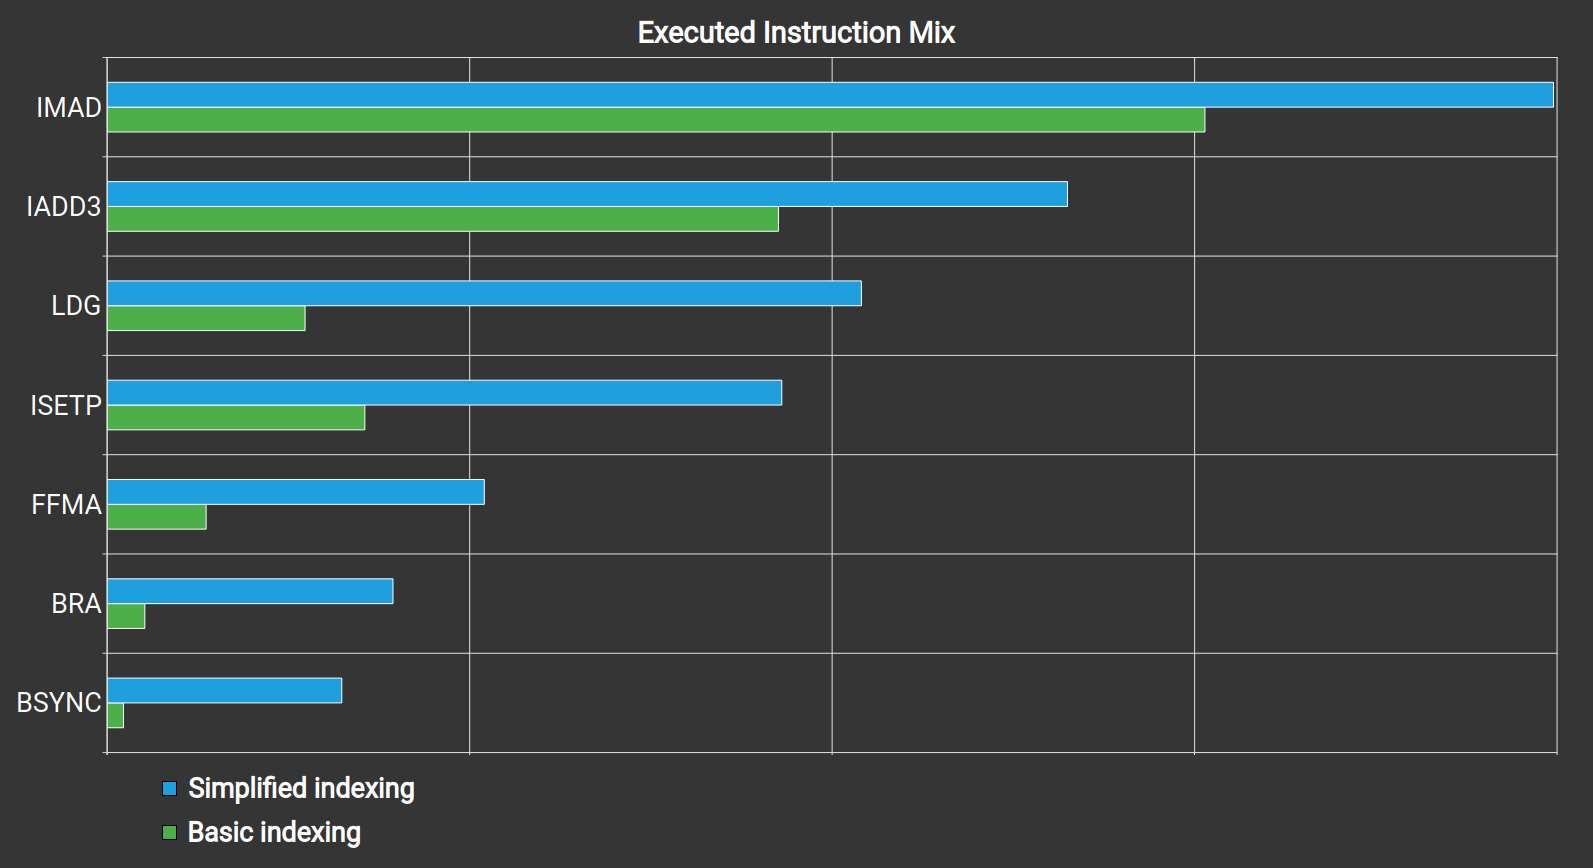
\includegraphics[width=0.8\textwidth]{executed_instructions_simplified_indexing.png}
	\caption{Comparison of the instruction mix executed by basic and simplified indexing.}
	\label{fig:executed_instructions_simplified_indexing}
\end{figure}

\begin{figure}[ht]
	\centering
	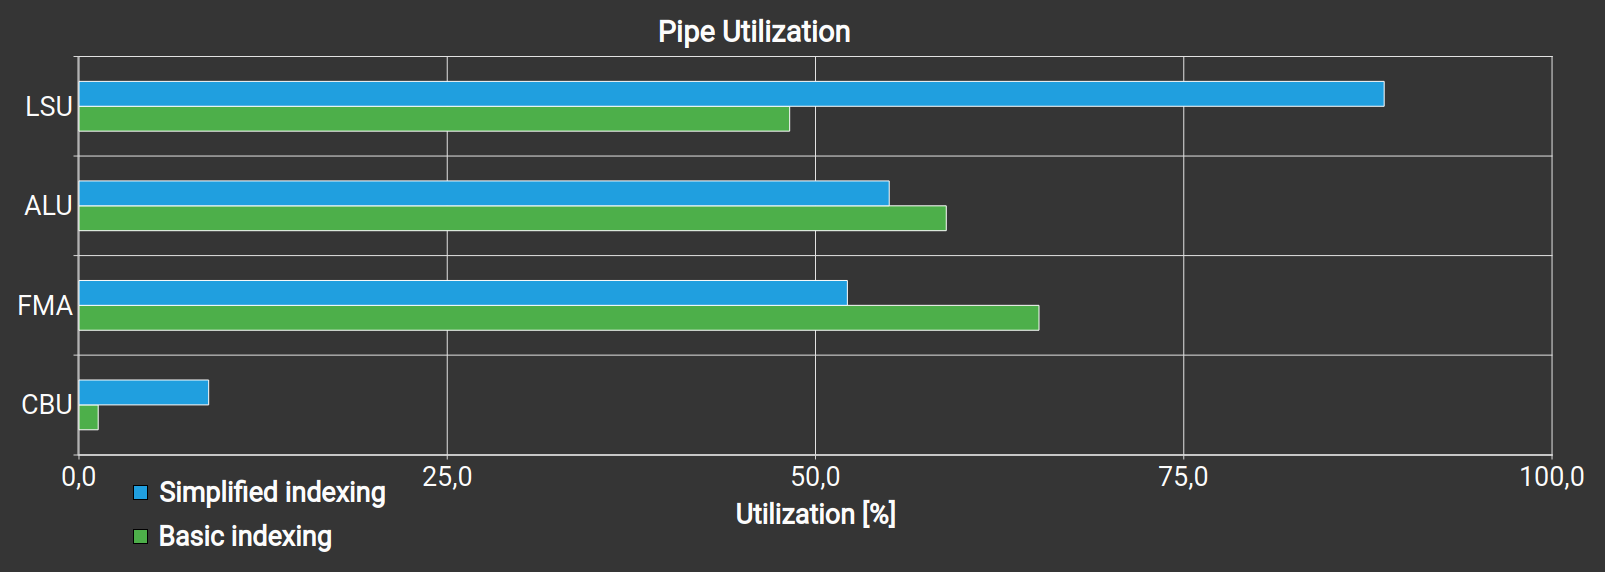
\includegraphics[width=0.8\textwidth]{pipeline_utilization_simplified_indexing.png}
	\caption{Comparison of pipeline utilization of the basic and simplified indexing.}
	\label{fig:pipeline_utilization_simplified_indexing}
\end{figure}

The effects of different pipeline utilization can also be seen in Figure \ref{fig:warp_state_simplified_indexing}. Warps of basic indexing algorithm are mostly stalled due to not being selected, i.e. there are multiple eligible warps and only one of them can be issued. This indicates that there may be too many warps for the size of the GPU. As these benchmarks were run on a RTX 2060 mobile, which is a rather small GPU, this was to be expected. The other main reason of warp stall is \texttt{Stall Math Pipe Throttle}, which is caused by the high utilization of \textit{ALU} and \textit{FMA} pipelines. These pipelines are responsible for computing the indices and the actual results of cross-correlation, which represent the useful work done by the GPU.

Simple indexing warps on the other hand are more often stalled on the \texttt{Stall Wait}, which represents warps waiting for a fixed latency execution dependency, i.e. a data dependency between two instructions or an instruction dependency on predicate computation. We can also see noticeable increase in stalls due to access to global memory (\texttt{Stall Long Scoreboard} and \texttt{Stall LG Throttle}) together with stalls due to branching. This is consistent with the properties of simple indexing described above.

\begin{figure}[ht]
	\centering
	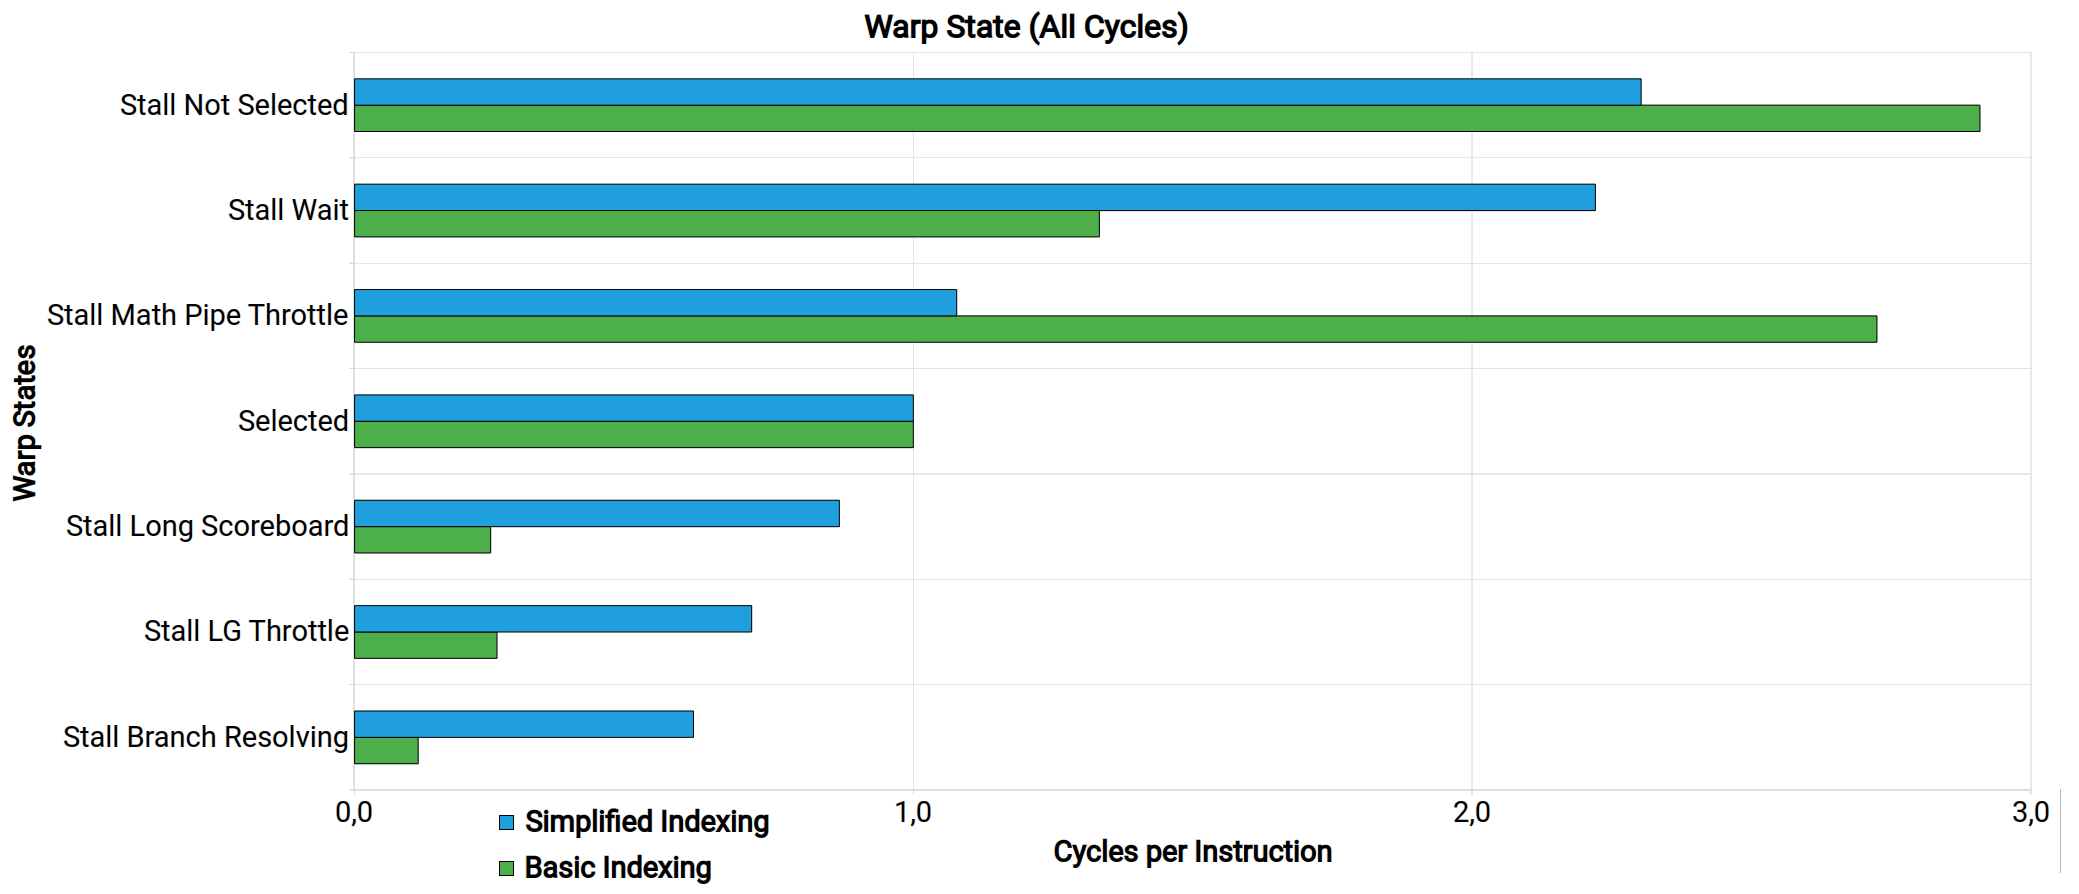
\includegraphics[width=0.8\textwidth]{warp_state_simplified_indexing.png}
	\caption{Comparison of warp stall reasons between the basic and simplified indexing.}
	\label{fig:warp_state_simplified_indexing}
\end{figure}

\subsection{Shared memory}
\label{sec:warp_per_shift_shared_mem}

This optimalization takes inspiration from the warp shuffle algorithm and its multirow optimalization. Instead of sharing input values by shifting and broadcasting across threads of a warp, we load input values into shared memory and reuse them by all warps of the thread block.

% Warps of a block compute consecutive shifts in Y axis
Warps of a given thread block compute consecutive shifts in the \textit{y} axis, as can be seen in Figure \ref{fig:warp_per_shift_shared_mem_shifts}. This allows us to prevent bank conflicts, which are a major problem when using shared memory. Figure \ref{fig:warp_per_shift_shared_mem_overlaps_in_x} illustrates shared memory access if we were to assign shifts along the \textit{x} axis, with warp size 4 and 4 banks of shared memory. As we can see, this leads to strided access, where warps access blocks of consecutive values with a stride between the blocks. This is guaranteed to cause up to 32 way bank conflicts, which would severely limit the shared memory throughput.

\begin{figure}[ht]
	\centering
	\def\svgwidth{\textwidth}
	% Must be relative to current directory
	% as input ignores graphicspath, which is
	% only for includegraphics{}
	\input{./img/warp_per_shift-SharedMemAlongY.pdf_tex}
	\caption{First two iterations with shifts assigned to warps along the \textit{y} axis.}
	\label{fig:warp_per_shift_shared_mem_shifts}
\end{figure}

When assigning shifts along the \textit{y} axis, all warps of a thread block compute the same shift in the \textit{x} axis, which corresponds to the same row size of the overlapping submatrices, as can be seen in Figure \ref{fig:warp_per_shift_shared_mem_shifts}. The only difference is the number of rows each overlapping submatrix contains. This leads to different starting and ending offsets for each of the warps, but allows us to utilize perfect linear access to shared memory, leading to optimal throughput. Left input matrix is accessed independently from the right input matrix, so sharing banks between the matrices does not lead to bank conflicts.

When loading data to shared memory, all warps of a block cooperate together to load the union of submatrices of all warps into shared memory. The union is divided into column groups of size \texttt{shared\_mem\_row\_size} columns, where \texttt{shared\_mem\_row\_size} is a runtime algorithm argument. These column groups are processed sequentially. The column groups can be seen in Figure \ref{fig:shared_mem_preload_offset}. This is also a place for further parallelization similar to work distribution, where each column group can be processed independently and in parallel, which is described in Section \ref{sec:column_group_per_worker}.

As in the warp shuffle algorithm, the data from the left matrix is loaded into two buffers which serve as a ring buffer. We first preload the bottom part of the buffer before the start of the outer loop. We have to limit the range of rows preloaded into the bottom left buffer to those which overlap with the rows loaded into the right buffer in the first iteration. If we were to preload the whole bottom left buffer, as can be seen in Figure \ref{fig:shared_mem_preload_offset}, we would encounter a situation where data loaded into the right buffer in the second iteration requires data preloaded into the bottom left buffer which are already overwritten.

\begin{figure}[ht]
	\centering
	\def\svgwidth{\textwidth}
	% Must be relative to current directory
	% as input ignores graphicspath, which is
	% only for includegraphics{}
	\input{./img/warp_per_shift-SharedMemPreload.pdf_tex}
	\caption{Why shared memory preload without offset does not work.}
	\label{fig:shared_mem_preload_offset}
\end{figure}

The size of each buffer is $shared\_mem\_row\_size * shared\_mem\_rows$, where \textit{shared\_mem\_rows} is another runtime algorithm parameter. This parameter has to be greater than or equal to the number of warps (and consequently computed shifts) per block.

The whole algorithm is described by the following pseudocode:
\begin{lstlisting}[]

FOR each column group
	preload bottom part of left buffer

	FOR rows of overlap with step shared_mem_rows
		load top part of left buffer
		load right buffer

		sync thread block

		compute bottom left buffer with right buffer
		compute top left buffer with right buffer

		swap top and bottom left buffer
		sync thread block
	END FOR
END FOR

\end{lstlisting}

Computation of left buffer half with right buffer computes the range of rows loaded into the two buffers which overlap in the shift assigned to the current warp. This gives two continuous ranges of the same size, one in left buffer half and one in the right buffer. Corresponding elements have to be multiplied and the result added to intermediate sum kept by each thread. After we process the whole overlapping submatrix, the intermediate sums in each thread are collected using the \texttt{reduce} function provided by Cooperative Groups API and the output is written to the output matrix by the first thread of the warp.


\begin{figure}[ht]
	\centering
	\def\svgwidth{0.5\textwidth}
	% Must be relative to current directory
	% as input ignores graphicspath, which is
	% only for includegraphics{}
	\input{./img/warp_per_shift-SharedMemAlongX.pdf_tex}
	\caption{Bank conflicts with shifts assigned to warps along the \textit{x} axis.}
	\label{fig:warp_per_shift_shared_mem_overlaps_in_x}
\end{figure}


% 	Its basically very similar to multirow optimization, just with workers of warp size
% 	And because they are warp size, we can compute bounds for each and stop them whenever
%	we need without thread divergence
Even with the throughput of shared memory, the load from shared memory \textit{LDS} instructions become a bottleneck, as can be seen in Figure \ref{fig:warp_state_shared_mem}. The memory input/output stall is caused by the memory input/output queue being full. This queue handles special math instructions, dynamic branches and most importantly for us the shared memory access instructions.

\begin{figure}[ht]
	\centering
	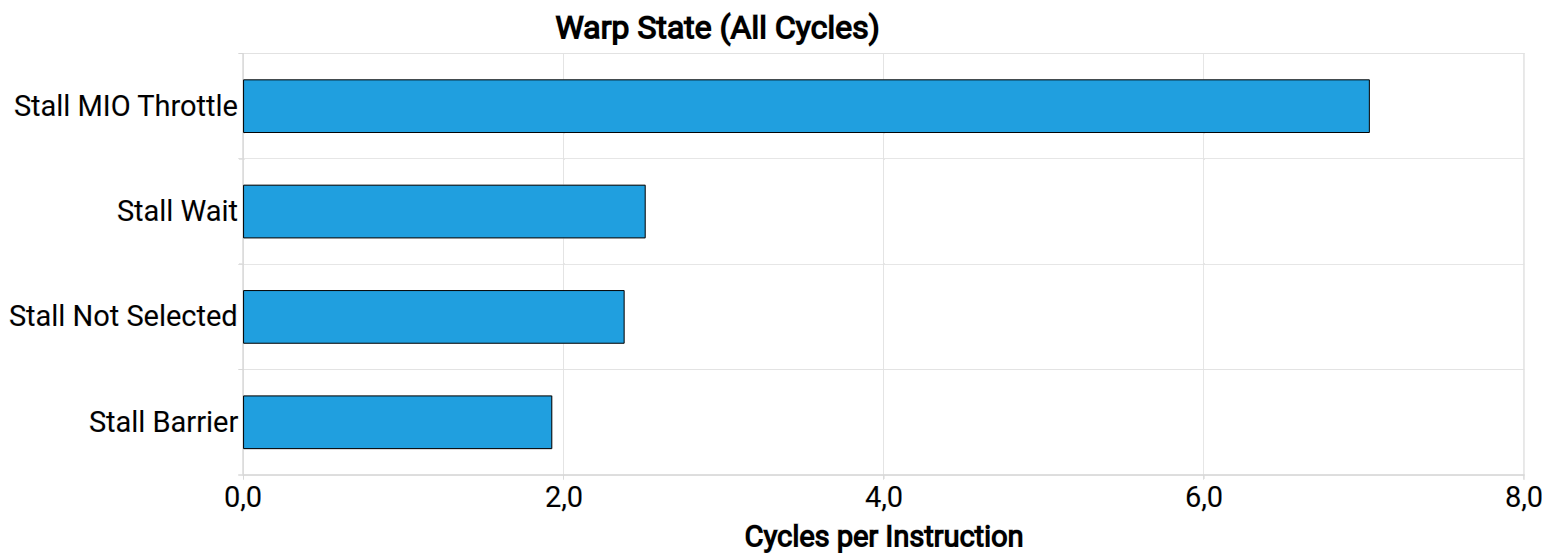
\includegraphics[width=0.8\textwidth]{warp_state_shared_mem.png}
	\caption{Memory input/output (MIO) stall caused by excessive shared memory access.}
	\label{fig:warp_state_shared_mem}
\end{figure}

\subsection{Loading data to shared memory}

When loading data to shared memory, we have a choice between two different access patterns, shown in Figure \ref{fig:shared_memory_loading_patterns}:
\begin{itemize}
	\item strided warps,
	\item continuous warps.
\end{itemize}

\begin{figure}[ht]
	\centering
	\def\svgwidth{0.6\textwidth}
	% Must be relative to current directory
	% as input ignores graphicspath, which is
	% only for includegraphics{}
	\input{./img/warp_per_shift-SharedMemLoading.pdf_tex}
	\caption{Difference between strided and continuous loading patterns.}
	\label{fig:shared_memory_loading_patterns}
\end{figure}

With strided warps, warp \textit{w} in iteration \textit{i} reads items based on the following formula:
\[ \left[i * block\_size + w * warp\_size, i * block\_size + (w + 1) * warp\_size\right) \]

With continuous warps, the whole block of data which is to be loaded is divided into equal parts, one for each warp. Each warp then loads the single continuous part of the data. The advantage compared to strided loads is that this access pattern should better utilize caches, as each warp does sequential access. The disadvantage is mainly in the fact that each warp will load some part of the data, even if the data is small and could be loaded by a subset of warps strided loading was used. For our input sizes and data access patterns, strided loading seems to be faster. % TODO: Benchmark results

\subsection{Shared memory with multiple right matrices}

Similarly to warp shuffle algorithm, we can increase the ratio of arithmetic instructions to shared memory loads by computing the same shift between a single left matrix and multiple right matrices. By reusing the data loaded from left matrix with multiple right matrices, we not only increase the ratio of arithmetic instructions, but also reduce the total number of loads from global memory and shared memory due to the reuse of data from the left matrix for computation of shifts of multiple right matrices. The effects of this optimization can be seen in Figures \ref{fig:executed_instructions_shared_mem} and \ref{fig:pipeline_utilization_shared_mem}. The number of shared memory load instructions (LDS) and memory access index computations using the integer multiply-add (IMAD) is significantly reduced. Even with this reduction, the utilization of the \textit{LSU} pipeline is still a bottleneck, most likely due to the reduced throughput of shared memory in the 7.5 Compute Capability we used for profiling. The higher utilization of \textit{FMA} pipeline hints at better performance, which will be shown in Section \ref{sec:results_shared_mem}.

\begin{figure}[ht]
	\centering
	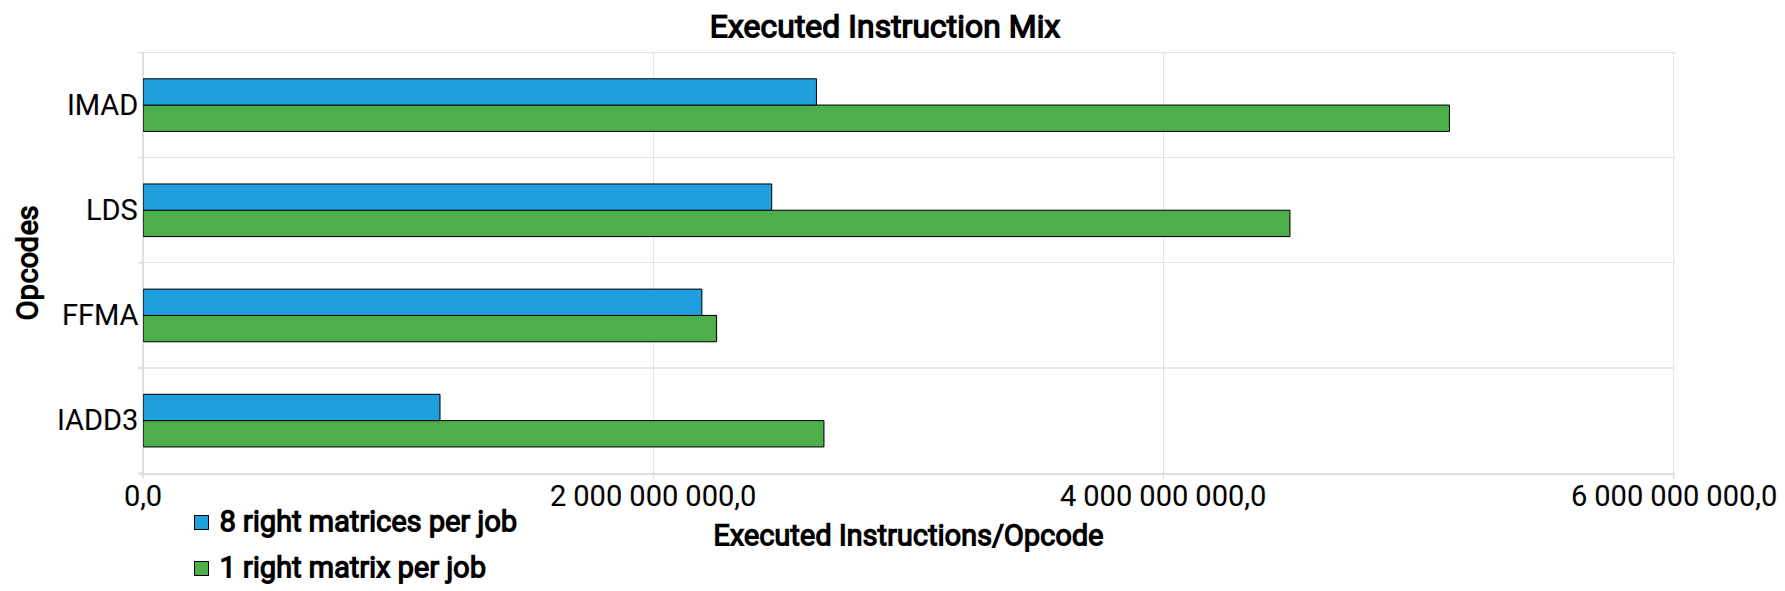
\includegraphics[width=0.8\textwidth]{executed_instructions_shared_mem.png}
	\caption{The effects of multiple right matrices optimization on executed instructions.}
	\label{fig:executed_instructions_shared_mem}
\end{figure}

\begin{figure}[ht]
	\centering
	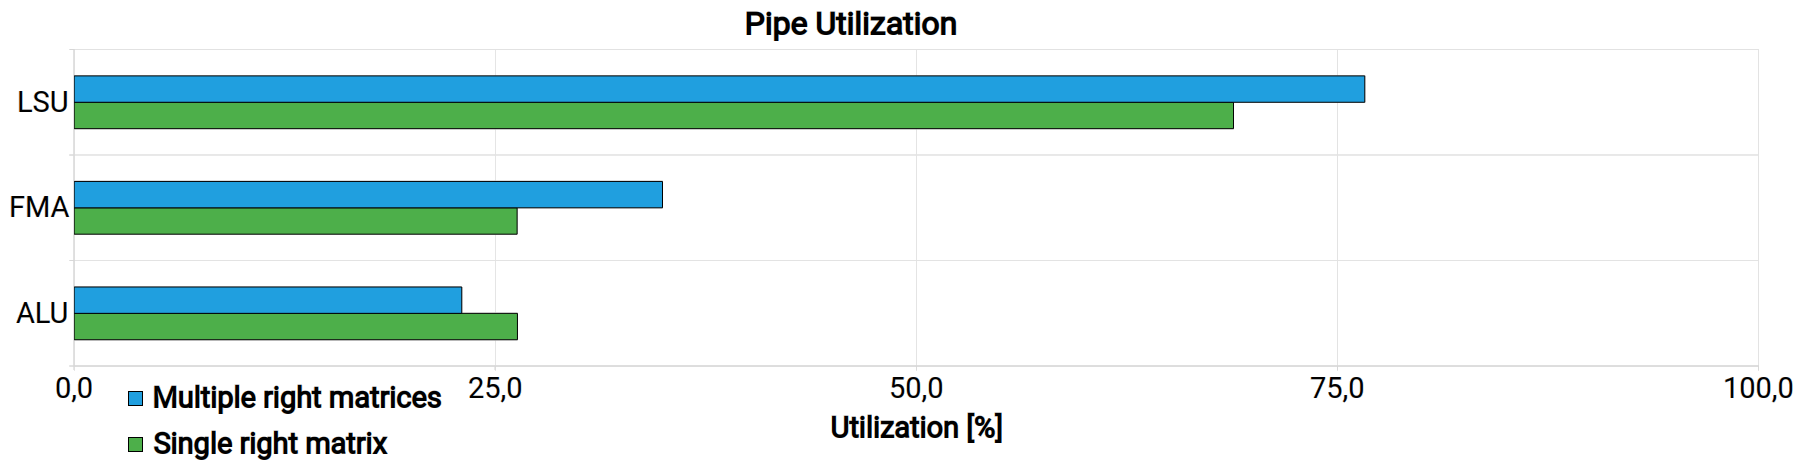
\includegraphics[width=0.8\textwidth]{pipeline_utilization_shared_mem.png}
	\caption{The effects of multiple right matrices optimization on pipeline utilization.}
	\label{fig:pipeline_utilization_shared_mem}
\end{figure}

\subsection{Shared memory with single column group per block}
\label{sec:column_group_per_worker}
As described in Section \ref{sec:warp_per_shift_shared_mem}, each column group processed by the shared memory optimization can be computed independently. This optimization borrows from the rectangle work distribution from Section \ref{sec:warp_shuffle_work_dist}, first computing the maximum number of column groups per shifts $m$ and then starting $m$ workers for each shift.

We utilize the \textit{z} dimension of the grid size to multiply the number of workers by $m$. Based on thread block \textit{z} index, each warp computes its assigned column group of the given shift. Redundant workers are stopped after this computation. The overlap bounds are computed to only include the assigned column group, after which the code from the original implementation with multiple column groups can be reused without any changes.

\subsection{Work distribution}

As described in Section \ref{sec:warp_shuffle_work_dist} with the warp shuffle algorithm, there are massive differences between work done by different workers in the basic algorithm. The implementation of this optimization is shared with the warp shuffle algorithm, only difference being the size of workers. We can choose from the \texttt{triangle} or \texttt{rectangle} distributions and set the maximum number of rows processed by a worker.

In our benchmarks using RTX 2060 GPU, this optimization was only beneficial for inputs smaller than 32 by 32, as can be seen in Figure \ref{fig:warp_per_shift_work_dist_local_results}. For larger inputs, the GPU is already saturated and with each warp processing a single shift, the workload per thread is already small enough that the work distribution does not bring much improvement. Additionally, without the use of shared memory described in Section \ref{sec:warp_per_shift_shared_mem}, the added load onto global memory makes this implementation slower for larger inputs.

With larger GPUs, the boundary where the benefits of increased occupancy are diminished by added strain onto global memory is moved onto larger inputs, as can be seen in Figure \ref{fig:warp_per_shift_work_dist_gpulab}. % TODO: Benchmark on GPU lab


% TODO: Maybe switch to kernel runtime from total computation time
\begin{figure}[ht]
	\centering
	\def\svgwidth{0.6\textwidth}
	% Must be relative to current directory
	% as input ignores graphicspath, which is
	% only for includegraphics{}
	\input{./img/warp_per_shift_work_dist_local_results.pdf_tex}
	\caption{Difference between strided and continuous loading patterns.}
	\label{fig:warp_per_shift_work_dist_local_results}
\end{figure}



\subsection{Block per shift}

Another step in increasing occupancy is to switch from warps as workers to whole thread blocks as workers. This can massively increase the number of threads started for given size of input, saturating the GPU even for smaller inputs.
The implementation is rather simple. The block index directly maps to the position in the output matrix and consequently to the shift computed by given block. We then compute the bounds of the overlapping submatrix corresponding with the shift computed by the current block and iterate over the overlapping elements using block stride loop. We then utilize \texttt{reduce} function provided by Cooperative Groups API to sum results in each warp, which are then stored into shared memory and  reduced again by warp 0. The final result is then stored in to the output matrix.

Based on our testing with RTX 2060, warps per shift with work distribution was enough to saturate the GPU even for smallest inputs. For inputs of size 32 by 32 or above, even work distribution was not required to saturate the GPU and the simplicity of the simplified algorithm and starts to take over, as can be seen in Figure \ref{fig:block_per_shift_local_results}. 

\begin{figure}[ht]
	\centering
	\def\svgwidth{0.6\textwidth}
	% Must be relative to current directory
	% as input ignores graphicspath, which is
	% only for includegraphics{}
	\input{./img/block_per_shift_local_results.pdf_tex}
	\caption{Difference between strided and continuous loading patterns.}
	\label{fig:block_per_shift_local_results}
\end{figure}

For larger GPUs, this implementation may be beneficial, but may also suffer from the low workload per thread, unbalanced workload between workers and no data reuse.

% TODO: Benchmark on GPULab


